\documentclass[tikz,border=6pt]{standalone}
\usepackage{ctex}
\usepackage{amsmath}
\usetikzlibrary{calc, arrows.meta}

\begin{document}
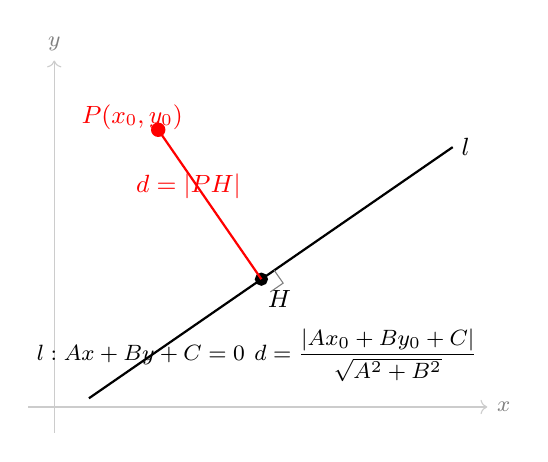
\begin{tikzpicture}[
  scale=1.1, thick,
]

% 坐标轴（参考）
\draw[gray!40, thin, ->] (-0.3, 0) -- (5.0, 0) node[right, font=\footnotesize, gray] {$x$};
\draw[gray!40, thin, ->] (0, -0.3) -- (0, 4.0) node[above, font=\footnotesize, gray] {$y$};

% 直线 l：从 (0.5, 0.2) 到 (4.5, 3.0)，斜率约 0.7
\draw[black, thick] (0.4, 0.1) -- (4.6, 3.0);
\node[font=\small] at (4.75, 3.0) {$l$};

% 点 P（不在直线上，位于直线左上方）
\coordinate (P) at (1.2, 3.2);
\filldraw[red, thick] (P) circle (2pt);
\node[font=\small, red] at (0.9, 3.35) {$P(x_0,y_0)$};

% 垂足 H：P 到 l 的垂足
% l 方向向量 (4.1, 2.9)/|...|；法向量 (-2.9, 4.1)
% l 参数：P + t*(法向量) 与 l 相交
% l: 过 (0.4,0.1) 方向 (4.2, 2.9)，单位化...
% 计算：l 过 A=(0.4,0.1), 方向 d=(4.2,2.9)
% H = A + t*d，使 (H-P) 垂直 d
% (A + t*d - P)·d = 0
% t = (P-A)·d / |d|^2
% P-A = (0.8, 3.1), d=(4.2,2.9)
% (P-A)·d = 0.8*4.2 + 3.1*2.9 = 3.36 + 8.99 = 12.35
% |d|^2 = 4.2^2+2.9^2 = 17.64+8.41 = 26.05
% t = 12.35/26.05 ≈ 0.4741
% H = (0.4 + 0.4741*4.2, 0.1 + 0.4741*2.9) = (0.4+1.991, 0.1+1.375) = (2.391, 1.475)
\coordinate (H) at (2.391, 1.475);
\filldraw[black] (H) circle (1.8pt);
\node[font=\small] at (2.6, 1.25) {$H$};

% 垂线 PH（红色，待求距离）
\draw[red, thick] (P) -- (H);

% 直角标记
% 垂线方向（P到H）: (2.391-1.2, 1.475-3.2) = (1.191, -1.725), 单位化
% 直线方向: (4.2, 2.9), 单位化
% 直角标记边长 0.18
\coordinate (d_unit) at ({4.2/5.102}, {2.9/5.102}); % 5.102=sqrt(26.05)
\coordinate (PH_unit) at ({1.191/2.082}, {-1.725/2.082}); % 2.082=|PH|

\draw[gray, thin]
  ($(H) + 0.18*(0.8228, 0.5684)$) --
  ($(H) + 0.18*(0.8228, 0.5684) + 0.18*(0.5721, -0.8202)$) --
  ($(H) + 0.18*(0.5721, -0.8202)$);

% 距离标注 d
\node[font=\small, red] at (1.55, 2.55) {$d = |PH|$};

% 距离公式
\node[font=\footnotesize, align=center] at (3.6, 0.6)
  {$d = \dfrac{|Ax_0+By_0+C|}{\sqrt{A^2+B^2}}$};

% 直线方程标注
\node[font=\footnotesize] at (1.0, 0.6) {$l: Ax+By+C=0$};

\end{tikzpicture}
\end{document}
